\documentclass[paper=a4, twoside=false, fontsize=12pt, parskip=half,
                bibliography=totoc, listof=totoc]{scrbook}

% General packages
\usepackage{sourdough}

% Basic attributes
\author{Hendrik Kleinwächter}
\title{The Sourdough Framework}

\begin{document}
\thispagestyle{empty}
\setlength{\unitlength}{1mm}
\noindent\begin{picture}(0,0)(1,-1)
\put(-16.3,-265){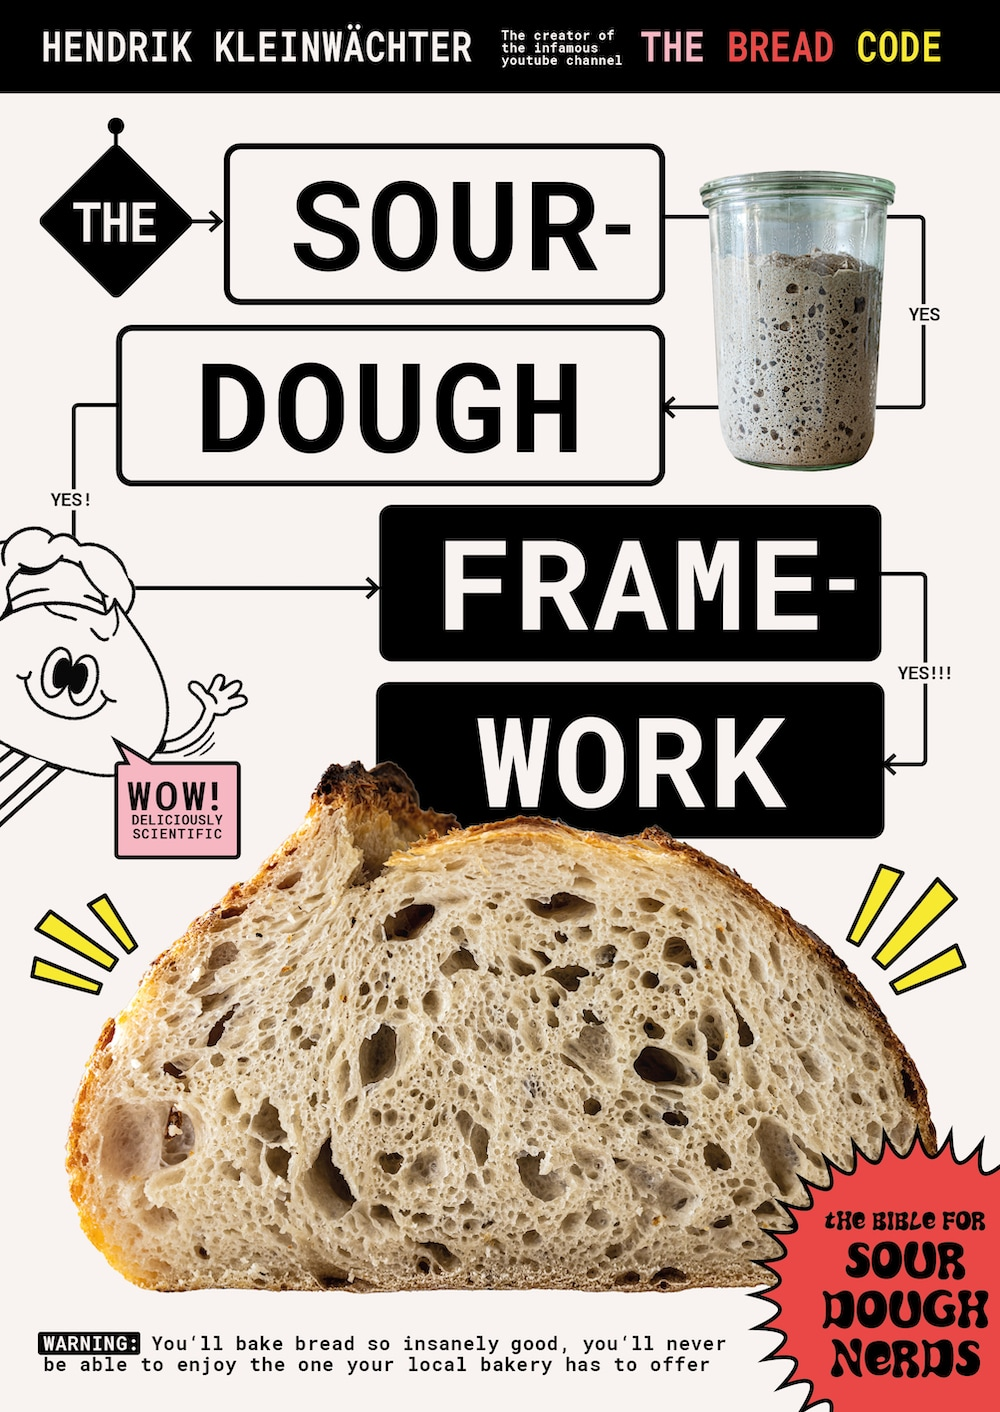
\includegraphics[width=1.33\linewidth]{cover/cover-page.jpg}}
\end{picture}

\newpage
\thispagestyle{empty}

\rule{1pt}{\textheight} % Vertical line
 % Whitespace between the vertical line and title page text
\hspace{0.05\textwidth}
 % Paragraph box for holding the title page text, adjust the width to move the
% title page left or right on the page
%\raggedleft%
\parbox[b]{0.75\textwidth}{%
{\Huge\bfseries The Sourdough Framework}\\[2\baselineskip] % Title
{\large\textit{Version: \today}}\\[4\baselineskip]
{\Large\textsc{Hendrik Kleinwächter}} % Author name, lower case for consistent small caps

% Whitespace between the title block and the copyright text
\vspace{0.5\textheight}

{\noindent The full source code for the book is available at \\
\url{https://github.com/hendricius/the-sourdough-framework/} under MIT
license. Do not hesitate to report mistakes or sug\-gestions for
improvements. A hardcover version of the book is also available. More information here:
\url{https://www.breadco.de/hardcover-book}}\\[\baselineskip]
}

\titlepage

{%
\hypersetup{hidelinks}
\ifdefined\HCode\else\tableofcontents\fi
}

\chapter{ebook problems}
Dès Noël, où un zéphyr haï me vêt de glaçons würmiens, je dîne d’exquis rôtis
de bœuf au kir, à l’aÿ d’âge mûr, \&cætera.
Jörg bäckt quasi zwei Haxenfüße vom Wildpony.

\begin{flowchart}[!htb]
\begin{center}
  \begin{tikzpicture}[node distance = 3cm, auto]
  \node [block] (heat_oven) {\footnotesize Preheat DO to  \qty{230}{\degreeCelsius} (\qty{446}{\degF}) for 30~minutes};
  \node [block, right of=heat_oven] (remove_oven) {\footnotesize Remove DO from oven };
  \node [block, right of=remove_oven] (open_load_dough) {\footnotesize Open DO \& load your dough};
  \node [block, right of=open_load_dough] (score) {\footnotesize Score your dough};
  \node [block, right of=score] (spritz) {\footnotesize Spritz dough with water};
  \node [block, below of=spritz] (close) {\footnotesize Close DO};
  \node [block, left of=close] (back_oven) {\footnotesize Place DO back in oven};
  \node [block, left of=back_oven] (bake) {\footnotesize Bake 30~minutes at \qty{230}{\degreeCelsius} (\qty{446}{\degF})};
  \node [block, below of=heat_oven] (wait_5_minutes) {\footnotesize Wait 5 minutes};
  \node [decision, below of=wait_5_minutes, node distance=4cm] (is_ready_check) {\footnotesize Core temperature \qty{92}{\degreeCelsius} (\qty{197}{\degF})?};
  \node [block, right of=is_ready_check, node distance=4cm] (remove_do_lid) {\footnotesize Remove DO lid};
  \node [block, right of=wait_5_minutes] (test_temperature_again) {\footnotesize Test core temperature again};
  \node [decision, right of=remove_do_lid, node distance=4cm] (dark_enough_decision) {\footnotesize Crust color dark enough?};
  \node [block, below of=dark_enough_decision] (finish_baking) {\footnotesize Bread is finished};
  \node [block, below of=close] (test_crust_again) {\footnotesize Test crust color again};
  \node [block, below of=test_crust_again] (bake_5_more_minutes) {\footnotesize Bake another 5~minutes};
  \path [line] (heat_oven) -- (remove_oven);
  \path [line] (remove_oven) -- (open_load_dough);
  \path [line] (open_load_dough) -- (score);
  \path [line] (score) -- (spritz);
  \path [line] (spritz) -- (close);
  \path [line] (close) -- (back_oven);
  \path [line] (back_oven) -- (bake);
  \path [line] (bake) -- (is_ready_check);
  \path [line] (is_ready_check) -- node{yes} (remove_do_lid);
  \path [line] (is_ready_check) -- node{no} (wait_5_minutes);
  \path [line] (wait_5_minutes) -- (test_temperature_again);
  \path [line] (test_temperature_again) -- (is_ready_check);
  \path [line] (remove_do_lid) -- (dark_enough_decision);
  \path [line] (dark_enough_decision) -- node{yes} (finish_baking);
  \path [line] (dark_enough_decision) -- node{no} (bake_5_more_minutes);
  \path [line] (bake_5_more_minutes) -- (test_crust_again);
  \path [line] (test_crust_again) -- (dark_enough_decision);
\end{tikzpicture}

  \caption[Baking process with a dutch oven]{A visualization of the baking
      process using a dutch oven (DO). The dough is steamed for the first half
      of the bake and then baked without cover for the second half of the
      bake. The desired darkness and thickness of the crust depends on your
      personal preference. Some bakers prefer a lighter crust and others a
      darker.}%
  \label{fig:dutch-oven-process}
\end{center}
\end{flowchart}

At around  \qty{60}{\degreeCelsius} (\qty{140}{\degF}) the microbes in your
dough start to die.  There are rumors that until this happens the microbes
produce a lot of \ch{CO2}.

% Does not work
\begin{figure}[!htb]
\begin{center}
  \footnotesize
\schemestart
\chemfig{H-C(-[2]H)(-[6]H)-C(-[2]H)(-[6]H)-O(-[7]H)} \+
\chemfig{O_2} \arrow
\chemfig{H-C(-[2]H)(-[6]H)-C(=[1]O)-[7]O-H} \+
\chemfig{H_2O}
\schemestop

  \caption[Acetic acid creation]{Oxygen is required to create acetic
      acid~\cite{acetic+acid+production}.}%
  \label{fig:ethanol-oxidation}
\end{center}
\end{figure}

% Works
% Generate first with: cd figures && pdflatex fig-ethanol-oxidation-external.tex
\begin{figure}[!htb]
  \begin{center}
    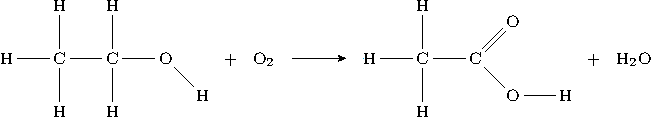
\includegraphics{figures/fig-ethanol-oxidation-external.pdf}
    \caption[Acetic acid creation]{Oxygen is required to create acetic
        acid~\cite{acetic+acid+production}.}%
  \end{center}
\end{figure}

% Does not work
\begin{figure}[!htb]
\begin{center}
  \begin{tikzpicture}
  % Draw horizontal line
  \draw[line width=1pt] (0,0) -- (\textwidth,0);

  % Define the width of each segment
  \pgfmathsetlengthmacro{\segmentwidth}{\textwidth/12}

  % Draw lines for the events, higher up so that they don't overflow the text
  % Placing the lines has been a bit manual work of trying different values
  % Maritime bacteria.

  \draw[line width=1pt] (2.8*\segmentwidth,1) -- (2.8*\segmentwidth,0.2);
  % Eukaryotes
  \draw[line width=1pt] (5.8*\segmentwidth,1.5) -- (5.8*\segmentwidth,0.2);
  % First bacteria on land
  \draw[line width=1pt] (9.1*\segmentwidth,-1.25) -- (9.1*\segmentwidth,-0.2);
  % Maritime fungi ancestors
  \draw[line width=1pt] (9.5*\segmentwidth,-2) -- (9.5*\segmentwidth,-0.2);
  % Fungi on land
  \draw[line width=1pt] (10.8*\segmentwidth,-2.75) -- (10.8*\segmentwidth,-0.2);
  % Yeasts on land
  \draw[line width=1pt] (11.1*\segmentwidth,-3.0) -- (11.1*\segmentwidth,-0.2);
  % First dinosaurs
  \draw[line width=1pt] (11.4*\segmentwidth,0.5) -- (11.4*\segmentwidth,0.2);
  % Pangea begins to rift apart
  \draw[line width=1pt] (11.6*\segmentwidth,1) -- (11.6*\segmentwidth,0.2);
  % Dinosaur extinction
  \draw[line width=1pt] (11.9*\segmentwidth,1.5) -- (11.9*\segmentwidth,0.2);
  % Additional line for dinosaurs since it is so close
  \draw[line width=1pt] (11.9*\segmentwidth,1.49) -- (11.70*\segmentwidth,1.85);

  % Special lines for december events since they are so close together
  \draw[line width=1pt] (12.0*\segmentwidth,3.0) -- (12.0*\segmentwidth,0.2);  % Main branch
  \draw[line width=1pt] (12.0*\segmentwidth,3.0) -- (11.75*\segmentwidth,2.5); % Branch to first humans
  \draw[line width=1pt] (12.0*\segmentwidth,3.0) -- (11.75*\segmentwidth,3.0); % Branch to Jordan
  % Move Pasteur down a bit so the lines look like they cross
  \draw[line width=1pt] (12.0*\segmentwidth,2.99) -- (11.75*\segmentwidth,3.5); % Branch to Pasteur

  % Draw months and month separators
  \foreach \i/\month in {0/Jan, 1/Feb, 2/Mar, 3/Apr, 4/May, 5/Jun, 6/Jul, 7/Aug, 8/Sep, 9/Oct, 10/Nov, 11/Dec} {
      % Separators
      \draw[line width=1pt] (\i*\segmentwidth,0.1) -- (\i*\segmentwidth,-0.1);
      % Month names
      \node[timeline_event, below] at ({(\i+0.5)*\segmentwidth},-0.1) {\month};
  }
  \draw[line width=1pt] (\textwidth,0.1) -- (\textwidth,-0.1);

  % Full timeline width for billion years
  \draw[stealth-stealth, line width=1pt] (0,-3.8) -- node[midway, timeline_timespan] {4.45 billion years} (\textwidth,-3.8);

  % Indicator for the period of 3 months = 1.1 billion years
  \draw[stealth-stealth, line width=1pt] (0,-1.0) -- node[midway, timeline_timespan] {1.11 billion years} ({\segmentwidth * 3},-1.0);

  % Place events on the timeline with dates using the timeline_event style
  % As a calculation I used (4.54 billion years / 12 months = 0.3785 billion years/month.
  \node[timeline_event, above] at (2.5*\segmentwidth,1) {Mar 25:~First maritime bacteria and archae};
  \node[timeline_event, above] at (4.50*\segmentwidth,1.5) {June 25:~First organisms with nuklei (eukaryotes)};
  \node[timeline_event, above] at (7.8*\segmentwidth,-1.5) {Oct 4:~First bacteria on land};
  \node[timeline_event, above] at (8.0*\segmentwidth,-2.25) {Oct 15:~First maritime ancestors of fungi};
  \node[timeline_event, above] at (9.7*\segmentwidth,-2.75) {Nov 24:~Fungi on land};
  \node[timeline_event, above] at (10.5*\segmentwidth,-3.25) {Dec 3:~Yeasts on land};
  \node[timeline_event, above] at (10.2*\segmentwidth,0.5) {Dec 14:~First dinosaurs};
  \node[timeline_event, above] at (9.8*\segmentwidth,1) {Dec 17:~Pangea begins to rift apart};
  \node[timeline_event, above] at (10.15*\segmentwidth,1.5) {Dec 29:~Dinosaurs go extinct};
  \node[timeline_event, above, anchor=east, align=right] at (11.75*\segmentwidth,2.5) {Dec 31:~First humans};
  \node[timeline_event, above, anchor=east, align=right] at (11.75*\segmentwidth,3.0) {Dec 31:~Sourdough in Jordan (23:59:55)};
  \node[timeline_event, above, anchor=east, align=right] at (11.75*\segmentwidth,3.5) {Dec 31:~Louis Pasteur isolated yeast (23:59:59)};

\end{tikzpicture}

  \caption[Sourdough microbiology timeline]{Timeline giberrish on website}%
\end{center}
\end{figure}

% Works
% In this case generate the graphic with pdflatex first: cd figures && pdflatex fig-life-planet-sourdough-timeline-external.pdf
\begin{figure}[!htb]
  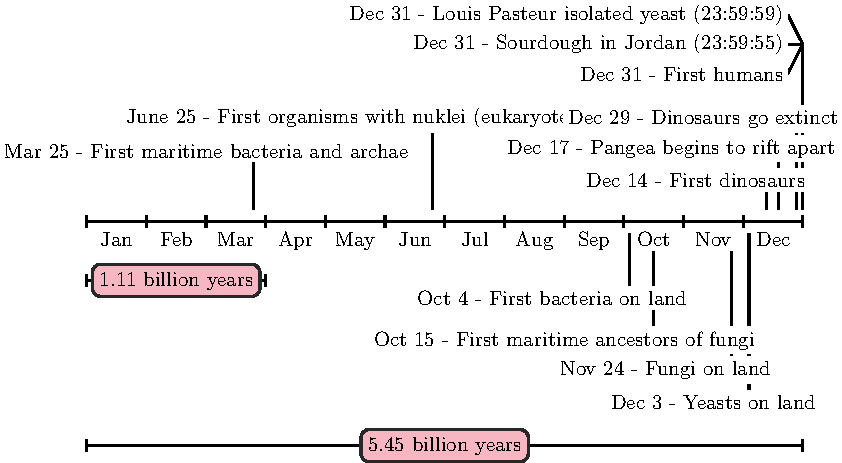
\includegraphics{figures/fig-life-planet-sourdough-timeline-external.pdf}
  \caption[Sourdough microbiology timeline]{Timeline works embedded as pdf}%
\end{figure}

\begin{figure}[!htb]
  \includegraphics[width=\textwidth]{baking-experiment-temperatures.png}
  \caption[Surface temperature for different steaming methods]{png file}
\end{figure}

\begin{figure}[!htb]
  \includegraphics[width=\textwidth]{baking-process-steam.jpg}
  \caption[Steam building with inverted tray]{jpg file}%
      \label{flc:inverted-tray}
\end{figure}
If you're a hobby brewer, you'll know that it's important to keep your beer at
certain temperatures to allow the different amylases to convert the contained
starches into sugar~\cite{beer+amylase}.
This test, called the \emph{Iodine Starch Test}, involves mixing iodine into
a sample of your brew and checking the color.

\begin{table}[!htb]
    \begin{center}
        \documentclass[tikz]{standalone}
\usepackage{tikz}
\usepackage{siunitx}
\DeclareSIUnit\degF{\text{°}F}

\definecolor{codeblue}{RGB}{69, 161, 248}
\definecolor{codegray}{RGB}{40, 40, 40}
\usetikzlibrary{shapes,arrows}
\tikzstyle{decision} = [diamond, draw, fill=codegray, text=white,
    text width=4.5em, text badly centered, node distance=3cm, inner sep=0pt]
\tikzstyle{block} = [rectangle, draw, fill=codeblue,  text=white,
    text width=5em, text centered, rounded corners, minimum height=4em]
\tikzstyle{line} = [draw, -latex']


\begin{document}
\begin{tabular}{llll}
\toprule
\textbf{Oven type}                                                         & \textbf{Plain (no tools)} & \textbf{Inverted tray} & \textbf{Dutch oven} \\ \midrule
Gas                                                                        & No                        & No                     & Yes                 \\ \midrule
\begin{tabular}[c]{@{}l@{}}Convection\\ (Fan always on)\end{tabular}       & No                        & No                     & Yes                 \\ \midrule
\begin{tabular}[c]{@{}l@{}}Convection\\ (Fan can be disabled)\end{tabular} & No                        & Yes                    & Yes                 \\ \midrule
Steam                                                                      &
Yes                       & Yes                    & Yes                 \\
\bottomrule
\end{tabular}
\end{document}

        \caption[Different oven types]{An overview of different oven types and their
            different baking methods.}
    \end{center}
\end{table}
{%
\hypersetup{hidelinks}
\listofflowcharts
\listoftables
\listoffigures
}
\printbibliography

\end{document}
